\documentclass{standalone}
\usepackage{tikz}
\usetikzlibrary{patterns, shadings}
\usepackage{color}
\begin{document}
	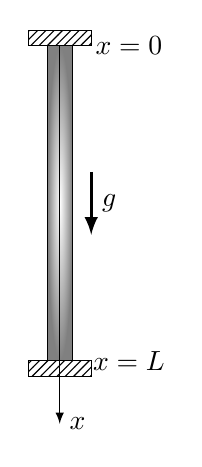
\begin{tikzpicture}[scale=.4]
		\draw[outer color=gray, inner color=white] (-.4, 0) rectangle (.4, 10);
		
		% Flechas
		\draw[-latex] (0, 10) -- (0, -2) node[right]{$x$};
		\draw[very thick, -latex] (1, 6) -- (1, 4) node[pos=.5, right]{$g$};
		
		% Apoyos
		\draw[pattern=north east lines] (-1, 10) rectangle (1, 10.5);
		\draw[pattern=north east lines] (-1, 0) rectangle (1, -.5);
		\node at (2.2, 10) {$x=0$};
		\node at (2.2, 0) {$x=L$};
	\end{tikzpicture}
\end{document}